%=============================================================================
\section{Zpracování informací}
%=============================================================================

\subsection{Strojové učení a dolování z dat (Data Mining)}

\subsubsection{Základní pojmy}

\paragraph{Umělá inteligence (AI)}

\textbf{AI} je obor informatiky zabývající se tvorbou systémů schopných vykonávat úkoly,
které by normálně vyžadovaly lidskou inteligenci -- jako je vnímání, uvažování, učení,
rozhodování nebo porozumění přirozenému jazyku.

Starší definice ``simulace lidského myšlení'' je nepřesná -- moderní AI systémy dosahují
inteligentního chování i metodami zcela odlišnými od lidské kognice (např. matice vah v
neuronové síti se nijak nepodobá lidskému mozku). Přesnější je říct:

\begin{center}\itshape
``AI = systém, který vnímá prostředí, zpracovává informace a jedná tak, aby dosáhl cíle.''
\end{center}

\paragraph{Rozdělení AI podle obecnosti}
\begin{itemize}
  \item \textbf{ANI (Narrow AI)} -- \textit{slabá AI}; zvládá jeden konkrétní úkol lépe než člověk;
    příklady: AlphaGo (Go), GPT (text), DALL-E (obrázky), spam filtr;
    \textbf{vše co dnes reálně existuje je ANI}
  \item \textbf{AGI (Artificial General Intelligence)} -- \textit{silná AI}; hypotetický systém
    schopný řešit libovolný intelektuální úkol jako člověk; dosud neexistuje
  \item \textbf{ASI (Artificial Super Intelligence)} -- hypotetická AI překonávající člověka ve
    všech oblastech; pouze spekulativní
\end{itemize}

\paragraph{Hierarchie pojmů: AI $\supset$ ML $\supset$ Deep Learning}

\begin{center}
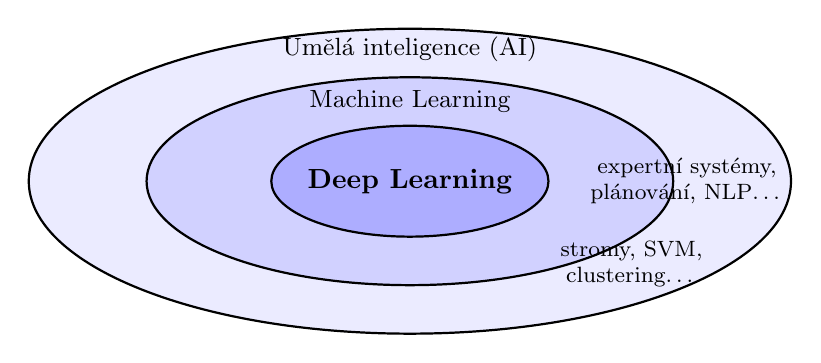
\begin{tikzpicture}[font=\small, scale=0.88]
  \draw[fill=blue!8,  thick] (0,0) ellipse (5.5cm and 2.2cm);
  \draw[fill=blue!18, thick] (0,0) ellipse (3.8cm and 1.5cm);
  \draw[fill=blue!32, thick] (0,0) ellipse (2.0cm and 0.8cm);
  \node[font=\bfseries] at (0,0) {Deep Learning};
  \node at (0, 1.15) {Machine Learning};
  \node at (0, 1.9) {Umělá inteligence (AI)};
  \node[font=\footnotesize, align=center] at (4.0, 0) {expertní systémy,\\plánování, NLP\ldots};
  \node[font=\footnotesize, align=center] at (3.2,-1.2) {stromy, SVM,\\clustering\ldots};
\end{tikzpicture}
\end{center}

\begin{itemize}
  \item \textbf{Strojové učení (ML)} -- podoblast AI; algoritmy, které se \textit{učí ze zkušenosti}
    (dat) bez explicitního programování pravidel; model sám odhalí vzory v datech
  \item \textbf{Hluboké učení (Deep Learning)} -- podoblast ML; vícevrstvé neuronové sítě;
    automaticky extrahuje příznaky (features) z raw dat (obrázkůy, textu, zvuku);
    příklady: CNN (počítačové vidění), Transformer (GPT, BERT)
  \item \textbf{Dolování dat (Data Mining)} -- průnik ML, statistiky a databázových technologií;
    zaměřen na odkrývání vzorů, korelací a trendů v (zejména databázových) datech;
    výsledky jsou interpretovatelné pro business
\end{itemize}

\paragraph{Typy strojového učení}
\begin{itemize}
  \item \textbf{Supervised learning (učení s učitelem)} -- trénovací data obsahují pár vstup-výstup
    (labely); model se naučí mapování; \textit{příklady:} klasifikace spamu, predikce ceny bytu,
    rozpoznávání obrazu
  \item \textbf{Unsupervised learning (bez učitele)} -- data bez labelů; model hledá strukturu sám;
    \textit{příklady:} segmentace zákazníků (clustering), detekce anomálií, doporučovací systémy
  \item \textbf{Reinforcement learning (posilované učení)} -- agent se učí interakcí s prostředím;
    dostává odměny za správné akce a tresty za špatné; \textit{příklady:} AlphaGo, autonomní řízení,
    optimalizace reklam
\end{itemize}

\subsubsection{CRISP-DM}

\textbf{CRISP-DM} (Cross-Industry Standard Process for Data Mining, 1999) je standardní metodika
popisující jak správně vést ML/data mining projekt od zadání po nasazení.

\textbf{Proč ji potřebujeme?} Bez struktury většina ML projektů ztroskotá na tom, že tým rovnou
skočí na modelování, zatímco 80\,\% práce tvoří příprava dat a pochopení problému.
CRISP-DM toto řeší -- říká ``nejdřív pochop problém, pak teprve modeluj''.

\textbf{Klíčová vlastnost:} metodika není lineární -- fáze se opakují a navzájem ovlivňují.
Typicky se mezi nimi iteruje vícekrát (např. po Evaluation zjistíme, že chybí data $\to$ zpět na Data Understanding).

\begin{figure}[H]
\centering
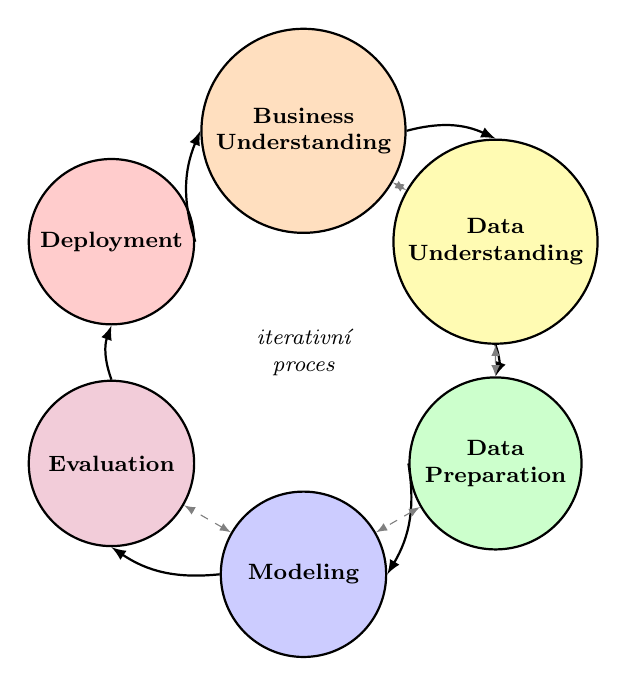
\begin{tikzpicture}[font=\small, scale=0.88,
  phase/.style={circle, draw, thick, minimum size=2.1cm, align=center, font=\footnotesize\bfseries},
  >=latex]
  % Six phases arranged in a circle
  \node[phase, fill=orange!25] (bu) at (90:3.2cm)  {Business\\Understanding};
  \node[phase, fill=yellow!30] (du) at (30:3.2cm)  {Data\\Understanding};
  \node[phase, fill=green!20]  (dp) at (330:3.2cm) {Data\\Preparation};
  \node[phase, fill=blue!20]   (mo) at (270:3.2cm) {Modeling};
  \node[phase, fill=purple!20] (ev) at (210:3.2cm) {Evaluation};
  \node[phase, fill=red!20]    (de) at (150:3.2cm) {Deployment};
  % Outer circular arrows
  \draw[->, thick] (bu.east)  to[bend left=20] (du.north);
  \draw[->, thick] (du.south) to[bend left=20] (dp.north);
  \draw[->, thick] (dp.west)  to[bend left=20] (mo.east);
  \draw[->, thick] (mo.west)  to[bend left=20] (ev.south);
  \draw[->, thick] (ev.north) to[bend left=20] (de.south);
  \draw[->, thick] (de.east)  to[bend left=20] (bu.west);
  % Inner bidirectional arrows (iterations)
  \draw[<->, dashed, gray] (bu) -- (du);
  \draw[<->, dashed, gray] (du) -- (dp);
  \draw[<->, dashed, gray] (dp) -- (mo);
  \draw[<->, dashed, gray] (mo) -- (ev);
  % Center label
  \node[align=center, font=\footnotesize\itshape] at (0,0) {iterativní\\proces};
\end{tikzpicture}
\caption{CRISP-DM -- šest iterativních fází}
\label{fig:crispdm}
\end{figure}

\textit{Praktický příklad: e-shop chce predikovat, který zákazník v příštím měsíci odejde (churn).}

\begin{enumerate}
  \item \textbf{Business Understanding -- co chceme dosáhnout?}
    \begin{itemize}
      \item Businessový cíl: snížit churn rate o 20\,\% cílenými retencními nabídkami
      \item Převod na ML problém: binární klasifikace -- zákazník odejde (1) nebo ne (0)
      \item Kritérium úspěchu: precision $\geq$ 70\,\% (nechceme zbytečně posílat slevy neodcházejícím)
    \end{itemize}

  \item \textbf{Data Understanding -- jaká data máme?}
    \begin{itemize}
      \item Zdrojová data: transakční DB (MS SQL), CRM systém, log webového chování
      \item EDA (Exploratory Data Analysis): distribuce proměnných, korelace, missing values
      \item Zjištění: 15\,\% zákazníků nemá vyplněný věk; churn je nevyvážený (5\,\% pozitivních)
    \end{itemize}

  \item \textbf{Data Preparation -- příprava pro model (80\,\% práce)}
    \begin{itemize}
      \item \textbf{Výběr příznaků (features):} počet nákupů za 3 měsíce, průměrná útrata,
        dny od posledního nákupu, počet stížností, kategorie produktů
      \item \textbf{Čištění:} imputace chybějícího věku (mediánem), odstranění duplicit
      \item \textbf{Transformace:} normalizace číselných hodnot, one-hot encoding kategorií
      \item \textbf{Řešení nebalance:} SMOTE (syntetické generování minority class)
    \end{itemize}

  \item \textbf{Modeling -- trénování modelu}
    \begin{itemize}
      \item Vyzkoušeny: logistická regrese (baseline), Random Forest, XGBoost
      \item Rozdělení dat: 70\,\% trénink / 15\,\% validace / 15\,\% test (nebo 10-fold CV)
      \item Hyperparameter tuning: Grid Search nebo Bayesian Optimization
      \item Nejlepší výsledek: XGBoost, AUC = 0.87
    \end{itemize}

  \item \textbf{Evaluation -- odpovídá model businessovým cílům?}
    \begin{itemize}
      \item Technická evaluace: Precision = 0.74, Recall = 0.61, F1 = 0.67, AUC = 0.87
      \item Businessová evaluace: identifikuje 61\,\% skutečných churnerů;
        splňuje cíl precision $\geq$ 70\,\%
      \item Rozhodnutí: model nasadit do pilotu pro segment Premium zákazníků
      \item \textit{Zpětná smyčka:} recall je nízký -- vrátíme se na Data Preparation a přidáme features
        z webového logu (navštívené stránky, čas na webu)
    \end{itemize}

  \item \textbf{Deployment -- model jde do produkce}
    \begin{itemize}
      \item Model zabalíme jako REST API (Python/Flask nebo FastAPI)
      \item Každý den se spustí pipeline: nová data $\to$ model $\to$ seznam zákazníků k oslovení
      \item CRM systém automaticky vytvoří kampaň s personalizovanou nabídkou
      \item Monitoring: sleduje se data drift (mění se vstupní data?) a model drift (klesá přesnost?)
    \end{itemize}
\end{enumerate}

\subsubsection{Rozhodovací stromy (Decision Trees)}

Hierarchická stromová struktura pro klasifikaci nebo regresi.

\paragraph{Struktura}
\begin{itemize}
  \item \textbf{Kořenový uzel} -- vstupní bod; první atribut pro větvení
  \item \textbf{Vnitřní uzly} -- testy podmínek na atributech
  \item \textbf{Větve} -- možné výsledky testu
  \item \textbf{Listy} -- výsledná třída nebo hodnota
\end{itemize}

\paragraph{Algoritmy}
\begin{itemize}
  \item \textbf{ID3, C4.5} -- kritérium informační gain (entropie)
  \item \textbf{CART} -- Gini impurity; produkuje binární stromy
  \item \textbf{Prořezávání (Pruning)} -- redukce přeučení (overfitting) odstraněním nerelevantních větví
\end{itemize}

\paragraph{Výhody a nevýhody}
\begin{itemize}
  \item \textbf{Výhody:} interpretovatelné, nevyžadují normalizaci, zvládají numerická i kategorická data
  \item \textbf{Nevýhody:} náchylné na přeučení, nestabilní (malá změna dat = jiný strom)
\end{itemize}

\begin{figure}[H]
  \centering
  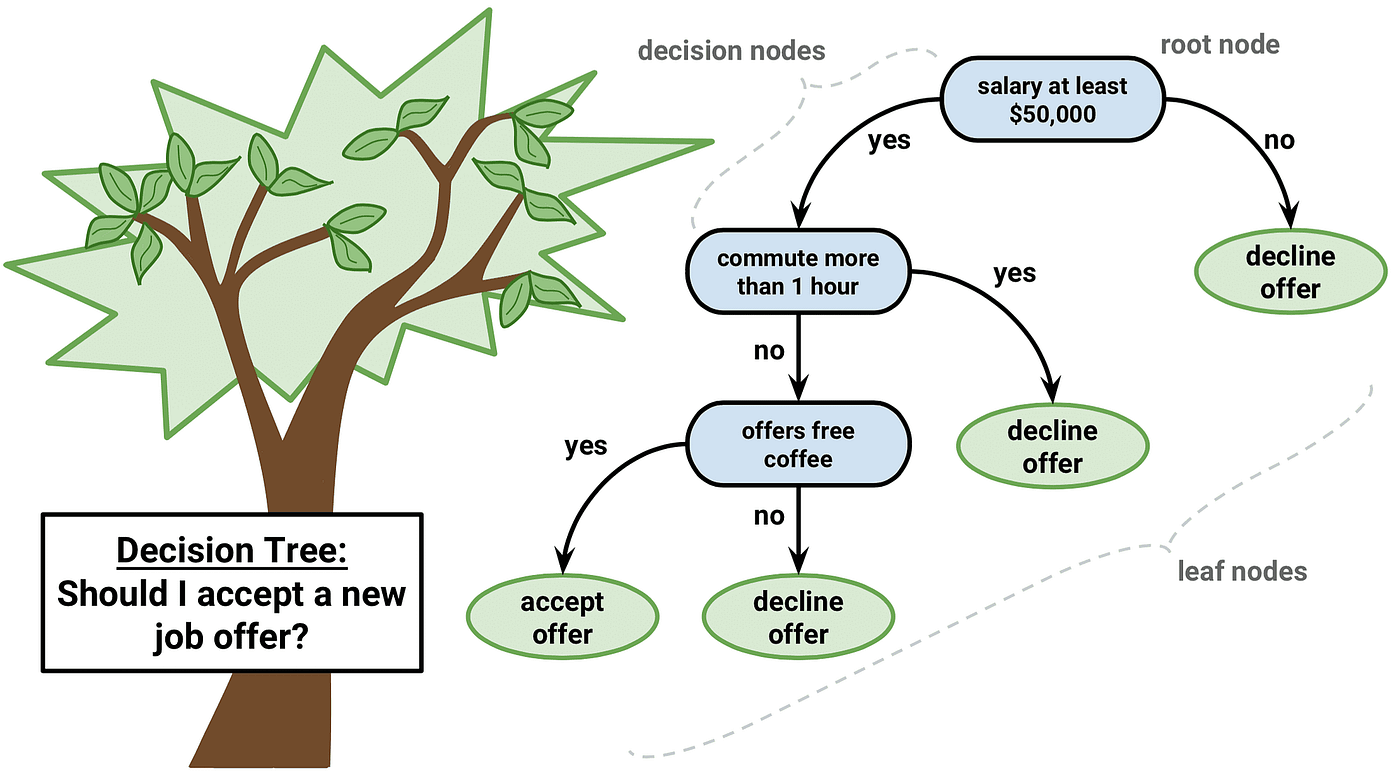
\includegraphics[width=0.7\textwidth]{img/decision-tree.png}
  \caption{Ukázka rozhodovacího stromu}
\end{figure}

\paragraph{Random Forest}
Ansamblová metoda; mnoho rozhodovacích stromů trénovaných na náhodných podmnožinách dat a atributů.
Výsledek: hlasování (klasifikace) nebo průměr (regrese). Redukuje overfitting.
\begin{itemize}
  \item \textbf{Klasifikace} -- každý strom hlasuje pro třídu (např. spam/ne-spam); výsledkem je třída s nejvíce hlasy.
  \item \textbf{Regrese} -- každý strom vrátí číselnou hodnotu (např. cenu nemovitosti); výsledkem je průměr všech předpovědí.
\end{itemize}
Proč redukuje overfitting: jeden strom se může přetrénovat na konkrétní data; průměrování/hlasování přes mnoho různorodých stromů tyto chyby vyruší.

\subsubsection{Clustering (Shlukování)}

Nesupervizovaná metoda; seskupení podobných objektů do skupin (clusterů).

\paragraph{K-Means}
\begin{enumerate}
  \item Inicializuj $k$ centroidů (náhodně nebo K-Means++)
  \item Přiřaď každý bod nejbližšímu centroidu (Euklidovská vzdálenost)
  \item Přepočítej centroidy jako průměr přiřazených bodů
  \item Opakuj 2--3 dokud se centroidy nepřestanou měnit
\end{enumerate}
Problém: nutno předem zvolit $k$; citlivý na odlehlé hodnoty; předpokládá kulové clustery.

\begin{figure}[H]
  \centering
  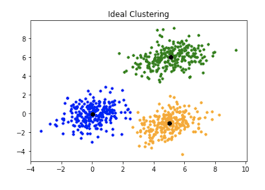
\includegraphics[width=0.7\textwidth]{img/kmeans.png}
  \caption{Ukázka K-Means clusteringu}
\end{figure}

\paragraph{Hierarchické shlukování}
\begin{itemize}
  \item \textbf{Agglomerativní} -- bottom-up; každý bod začíná jako vlastní cluster, postupně se spojují
  \item \textbf{Divisivní} -- top-down; začíná jedním clusterem, postupně se dělí
  \item Výstup: dendrogram (stromová struktura hierarchie)
\end{itemize}

\begin{figure}[H]
  \centering
  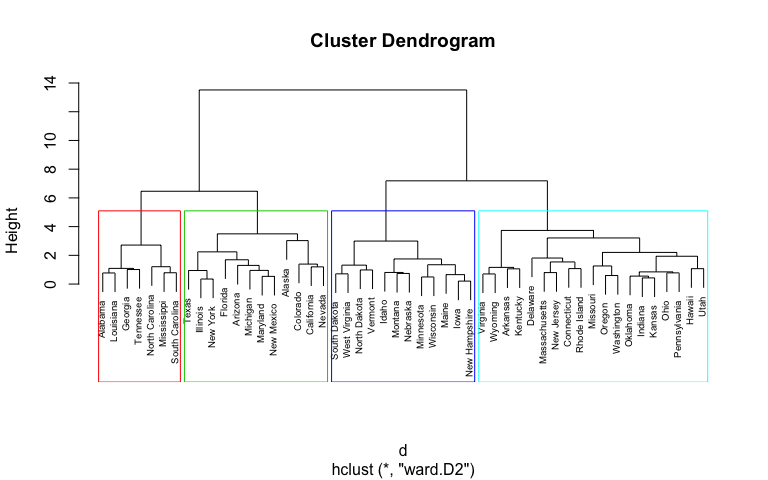
\includegraphics[width=0.7\textwidth]{img/hiercluster.png}
  \caption{Dendrogram hierarchického shlukování}
\end{figure}

\paragraph{DBSCAN}
Density-Based Spatial Clustering; clustery jako oblasti vysoké hustoty; zvládá libovolné tvary;
identifikuje outliers.

\subsubsection{Asociační pravidla}

Asociační pravidla hledají vztahy tvaru \textbf{``jestliže zákazník koupí A, koupí také B''}
v transakčních datech. Klasická aplikace: \textbf{analýza tržního košíku} (market basket analysis).

\textit{Příklad transakční databáze (5 nákupů):}
\begin{center}\footnotesize
\begin{tabular}{ll}
\toprule
\textbf{Transakce} & \textbf{Zakoupené položky} \\
\midrule
T1 & Pivo, Pleny, Chips \\
T2 & Pivo, Pleny \\
T3 & Pivo, Chips \\
T4 & Pleny, Chips, Džus \\
T5 & Pivo, Pleny, Chips, Džus \\
\bottomrule
\end{tabular}
\end{center}

\paragraph{Klíčové metriky -- intuitivně}

\textbf{1. Podpora (Support)} -- \textit{Jak běžná je tato kombinace celkově?}

$$\text{supp}(A \Rightarrow B) = \frac{\text{počet transakcí obsahujících A i B}}{\text{celkový počet transakcí}}$$

\textit{Příklad:} Pivo a Pleny se vyskytují společně v T1, T2, T5 -- tedy ve 3 z 5 transakcí:
$$\text{supp(Pivo} \Rightarrow \text{Pleny)} = \frac{3}{5} = 60\,\%$$
Nízká podpora = pravidlo platí jen zřídka (nezajímavé pro business).

\medskip
\textbf{2. Důvěra (Confidence)} -- \textit{Jak spolehlivé je pravidlo? Když zákazník koupí A, jak často koupí i B?}

$$\text{conf}(A \Rightarrow B) = \frac{\text{supp}(A \cup B)}{\text{supp}(A)} = P(B \mid A)$$

\textit{Příklad:} Pivo se vyskytuje v T1, T2, T3, T5 (4 transakce). Z nich Pleny jsou v T1, T2, T5 (3 transakce):
$$\text{conf(Pivo} \Rightarrow \text{Pleny)} = \frac{3}{4} = 75\,\%$$
Když zákazník koupí Pivo, v 75\,\% případů koupí také Pleny.
Vysoká důvěra \textbf{sama nestačí} -- pokud zákazníci kupují Pleny vždy (100\,\% podpora),
pak 75\,\% důvěra je vlastně \textit{horší} než náhodný výběr.

\medskip
\textbf{3. Lift} -- \textit{Je tato asociace opravdu zajímavá, nebo je to jen náhoda?}

$$\text{lift}(A \Rightarrow B) = \frac{\text{conf}(A \Rightarrow B)}{\text{supp}(B)}$$

Lift říká: \textit{o kolik více zákazníků koupí B díky tomu, že koupili A, oproti náhodnému výběru?}
\begin{itemize}
  \item \textbf{Lift $> 1$} -- pozitivní asociace; A skutečně pomáhá predikovat B; pravidlo je užitečné
  \item \textbf{Lift $= 1$} -- A a B jsou nezávislé; znalost A nepomáhá predikovat B
  \item \textbf{Lift $< 1$} -- negativní asociace; zákazníci kupující A méně pravděpodobně kupují B
\end{itemize}

\textit{Příklad:} Pleny jsou v T1, T2, T4, T5 -- supp(Pleny) = 4/5 = 80\,\%:
$$\text{lift(Pivo} \Rightarrow \text{Pleny)} = \frac{75\,\%}{80\,\%} = 0{,}94 < 1$$
Lift $< 1$ -- zákazníci kupující Pivo kupují Pleny \textit{méně} než průměr. Tato asociace není užitečná!

\begin{center}\footnotesize
\begin{tabular}{lllll}
\toprule
\textbf{Pravidlo} & \textbf{Support} & \textbf{Confidence} & \textbf{Lift} & \textbf{Závěr} \\
\midrule
Pivo $\Rightarrow$ Chips & 60\,\% & 75\,\% & 1.25 & Užitečné (lift $>$ 1) \\
Pivo $\Rightarrow$ Pleny & 60\,\% & 75\,\% & 0.94 & Nezajímavé (lift $<$ 1) \\
Pleny $\Rightarrow$ Chips & 60\,\% & 75\,\% & 1.25 & Užitečné \\
\bottomrule
\end{tabular}
\end{center}

\paragraph{Algoritmus Apriori -- k čemu slouží a jak funguje}

\textbf{Problém:} pro $n$ různých položek existuje $2^n$ možných kombinací -- pro supermarket
s 10\,000 produkty je to astronomické číslo. Nelze vyzkoušet všechny.

\textbf{Apriori} tento problém řeší chytrou zkratkou pomocí \textbf{anti-monotonní vlastnosti}:

\begin{tcolorbox}[colback=yellow!15, colframe=orange!60, title=Anti-monotonní vlastnost (klíčová myšlenka Apriori)]
Pokud je kombinace $\{A, B\}$ \textbf{nefrekventovaná} (podpora $<$ minSupport),
pak \textbf{každá nadmnožina} $\{A, B, C\}$, $\{A, B, D\}$, \ldots bude také nefrekventovaná.

$\Rightarrow$ Celé větve prostoru kombinací lze \textbf{odříznout bez prohledávání}.
\end{tcolorbox}

\textbf{Postup algoritmu:}
\begin{enumerate}
  \item Najdi všechny frekventované položky (supp $\geq$ minSupport): \{Pivo\}, \{Pleny\}, \{Chips\}\ldots
  \item Kombinuj dvojice a ověř jejich support: \{Pivo, Pleny\}, \{Pivo, Chips\}\ldots; \textbf{odřízni} nefrekventované
  \item Kombinuj trojice z frekventovaných dvojic\ldots; opakuj dokud nejsou žádné nové kombinace
  \item Z frekventovaných množin vygeneruj pravidla a vypočítej Confidence a Lift
\end{enumerate}

\textbf{K čemu je Apriori v praxi dobrý:}
\begin{itemize}
  \item \textbf{Merchandising / rozmístění zboží} -- zjistíš, že Pleny a Pivo se kupují dohromady
    $\to$ dej je do stejné uličky (nebo naopak do jiných, aby zákazník prošel celým obchodem)
  \item \textbf{Doporučovací systémy} -- ``zákazníci, kteří koupili X, také koupili Y''
    (Amazon, Netflix, Spotify to v základu takto dělají)
  \item \textbf{Křížový prodej (cross-selling)} -- banka zjistí, že klienti s hypotékou si brzy sjednají pojištění $\to$ proaktivní nabídka
  \item \textbf{Detekce podvodů} -- neobvyklé kombinace transakcí mohou signalizovat podvod
  \item \textbf{Analýza webového chování} -- které stránky se navštěvují spolu? $\to$ optimalizace navigace
\end{itemize}

\subsubsection{Hodnocení klasifikačních modelů}

\paragraph{Matice záměn (Confusion Matrix)}

\begin{center}
\begin{tabular}{lll}
\toprule
 & \textbf{Predikováno: ANO} & \textbf{Predikováno: NE} \\
\midrule
\textbf{Skutečnost: ANO} & TP (True Positive) & FN (False Negative) \\
\textbf{Skutečnost: NE}  & FP (False Positive) & TN (True Negative) \\
\bottomrule
\end{tabular}
\end{center}

\begin{itemize}
  \item \textbf{Accuracy} -- $\frac{TP+TN}{TP+TN+FP+FN}$ -- celková přesnost; kolik procent všech případů model klasifikoval správně. \textit{Pozor: zavádějící u nevyvážených dat -- model který vždy řekne „není spam" dosáhne 99\% accuracy, pokud je 99 \% e-mailů legitimních.}

  \item \textbf{Precision} -- $\frac{TP}{TP+FP}$ -- z \textit{všech které model označil jako pozitivní}, kolik jich skutečně pozitivní bylo. \\
    \textit{Příklad:} spamový filtr označil 100 e-mailů jako spam; z toho 90 bylo skutečně spam a 10 byly legitimní e-maily (FP). Precision = 90/100 = 90\%. \\
    \textit{Kdy je klíčová:} když je drahé mít falešný poplach -- nechceš posílat legitimní e-maily do spamu.

  \item \textbf{Recall (Sensitivity)} -- $\frac{TP}{TP+FN}$ -- z \textit{všech skutečně pozitivních případů}, kolik jich model našel. \\
    \textit{Příklad:} v e-mailech bylo 200 spamů; filtr zachytil 180 a 20 prošlo (FN). Recall = 180/200 = 90\%. \\
    \textit{Kdy je klíčová:} když je drahé zmeškat pozitivní případ -- diagnóza rakoviny (nechceš zmeškat ani jeden případ).

  \item \textbf{Precision vs Recall -- trade-off:} zvýšením prahu (model říká „pozitivní" jen když je velmi jistý) roste Precision ale klesá Recall a naopak.

  \item \textbf{F1 score} -- $2 \cdot \frac{Precision \cdot Recall}{Precision + Recall}$ -- harmonický průměr Precision a Recall; vyvážená metrika když ti záleží na obou; hodnota 0--1, čím vyšší tím lepší.

  \item \textbf{Specificity} -- $\frac{TN}{TN+FP}$ -- z reálných negativ, kolik bylo správně klasifikováno jako negativní.
\end{itemize}

\paragraph{ROC křivka a AUC}
\textbf{ROC křivka} (Receiver Operating Characteristic) zobrazuje, jak se mění Recall (TPR) vs falešně pozitivní míra (FPR = $\frac{FP}{FP+TN}$) při postupném snižování rozhodovacího prahu modelu. Každý bod na křivce odpovídá jednomu nastavení prahu.

\textbf{AUC} (Area Under Curve) -- plocha pod ROC křivkou; čím větší plocha, tím lepší model:
\begin{itemize}
  \item \textbf{AUC = 1.0} -- perfektní model; rozlišuje všechny pozitivní od negativních
  \item \textbf{AUC = 0.5} -- náhodný model (přímka); model neví nic
  \item \textbf{AUC = 0.8--0.9} -- dobrý model v praxi
\end{itemize}
\textit{Výhoda AUC:} nezávisí na konkrétním prahu -- hodnotí celkovou schopnost modelu rozlišovat třídy, ne jen jedno nastavení.

\paragraph{Metody ověřování modelů}
\begin{itemize}
  \item \textbf{Hold-out} -- rozdělení na trénovací (70--80\%) a testovací (20--30\%) množinu
  \item \textbf{K-fold cross-validation} -- data rozdělena na $k$ stejných částí; model natrénován na $k-1$ částech,
    testován na zbývající; opakováno $k$krát; výsledek = průměr; typicky $k=10$
  \item \textbf{Leave-one-out (LOO)} -- speciální případ k-fold kde $k=n$; nákladné, ale nejmenší bias
  \item \textbf{Bootstrap} -- opakované vzorkování s vracením; odhad variance modelu
\end{itemize}

\paragraph{Overfitting a underfitting}
\begin{itemize}
  \item \textbf{Overfitting (přeučení)} -- model se příliš přizpůsobil trénovacím datům; nízká chyba na trénování,
    vysoká na testování; řešení: regularizace, pruning, více dat, cross-validation
  \item \textbf{Underfitting (podučení)} -- model je příliš jednoduchý; vysoká chyba i na trénovacích datech;
    řešení: složitější model, více příznaků
\end{itemize}

%=============================================================================
\subsection{Ukládání a vyhledávání textových informací}
%=============================================================================

\subsubsection{Information Retrieval (IR)}

Disciplína zabývající se vyhledáváním nestrukturovaných informací (textu) v rozsáhlých kolekcích.
Klíčový pojem: \textbf{relevance} -- jak dobře dokument odpovídá dotazu.

\paragraph{Hodnocení IR systémů}
\begin{itemize}
  \item \textbf{Precision} -- z vrácených dokumentů, kolik je relevantních: $P = \frac{TP}{TP+FP}$
  \item \textbf{Recall} -- z relevantních dokumentů, kolik bylo vráceno: $R = \frac{TP}{TP+FN}$
  \item \textbf{F-measure:} $F_1 = 2 \cdot \frac{P \cdot R}{P + R}$ -- harmonický průměr precision a recall
\end{itemize}

\subsubsection{Booleovský model vyhledávání}

Nejstarší IR model. Dokumenty a dotazy reprezentovány jako množiny termů.

\begin{itemize}
  \item Dotaz je booleovský výraz: \texttt{informatika AND databáze AND NOT NoSQL}
  \item Dokument je relevantní, pokud splňuje booleovský výraz (1/0 -- binární relevance)
  \item \textbf{Výhody:} jednoduchost, přesnost formulace dotazu
  \item \textbf{Nevýhody:} žádné pořadí výsledků, výsledek je příliš citlivý na formulaci, žádná dílčí shoda
\end{itemize}

\paragraph{Rozšíření Booleovského modelu}
\begin{itemize}
  \item \textbf{Fuzzy model} -- stupně členství termů v dokumentu (0--1); termy s váhami
  \item \textbf{Geometrický model} -- dokumenty a dotazy jako vektory; relevance = vzdálenost
\end{itemize}

\subsubsection{Vektorový model (Vector Space Model)}

Každý dokument i každý dotaz se převede na \textbf{číselný vektor} -- jedno číslo (váha) pro každé
slovo v celém slovníku. Relevance dokumentu pro dotaz = \textbf{podobnost jejich vektorů}.

\textit{Pracovní příklad -- 3 dokumenty a 1 dotaz:}
\begin{center}\footnotesize
\begin{tabular}{ll}
\toprule
\textbf{ID} & \textbf{Text} \\
\midrule
D1 & ``databáze databáze SQL'' \\
D2 & ``databáze NoSQL'' \\
D3 & ``Python strojové učení'' \\
Q  & dotaz: ``databáze SQL'' \\
\bottomrule
\end{tabular}
\end{center}

\paragraph{TF-IDF váhování}
Váha termu $t$ v dokumentu $d$ říká: \textit{jak moc je toto slovo charakteristické pro tento dokument?}
$$w(t,d) = \underbrace{\text{TF}(t,d)}_{\text{četnost v doc.}} \cdot \underbrace{\text{IDF}(t)}_{\text{vzácnost ve sbírce}}$$

\begin{itemize}
  \item \textbf{TF (Term Frequency)} -- kolikrát se slovo vyskytuje v dokumentu; ``databáze'' v D1 = 2
  \item \textbf{IDF (Inverse Document Frequency)} $= \log\dfrac{N}{df(t)}$, kde $N$ = počet dokumentů,
    $df(t)$ = v kolika dokumentech se term vyskytuje.
    \begin{itemize}
      \item Čím více dokumentů slovo obsahuje, tím větší je $df(t)$, tím menší je podíl $N/df(t)$
            a tím nižší je IDF -- slovo není příliš rozlišovací.
      \item Běžná slova jako ``a'', ``the'' se vyskytují skoro ve všech dokumentech
            $\Rightarrow$ $df(t) \approx N$ $\Rightarrow$ $\log(N/N) = \log(1) = 0$
            $\Rightarrow$ váha blízká nule (filtrují se automaticky, bez stop-listu).
      \item Vzácné odborné slovo je třeba jen v jednom dokumentu
            $\Rightarrow$ $df(t) = 1$ $\Rightarrow$ $\log(N)$ -- maximální IDF, slovo je velmi charakteristické.
      \item Logaritmus tlumí extrémní rozdíly: sbírka s milionem dokumentů by bez něj dávala
            obrovská čísla; $\log$ je škáluje do rozumného rozsahu.
    \end{itemize}
\end{itemize}

\textit{Výpočet IDF pro náš příklad ($N = 3$):}
\begin{center}\footnotesize
\begin{tabular}{llll}
\toprule
\textbf{Term} & \textbf{$df(t)$} & \textbf{$\text{IDF} = \log(3/df)$} & \textbf{Interpretace} \\
\midrule
databáze & 2 & $\log(1{,}5) = 0{,}41$ & Střední vzácnost (ve 2/3 dokumentů) \\
SQL      & 1 & $\log(3{,}0) = 1{,}10$ & Vzácný (jen v D1) \\
NoSQL    & 1 & $\log(3{,}0) = 1{,}10$ & Vzácný (jen v D2) \\
Python   & 1 & $\log(3{,}0) = 1{,}10$ & Vzácný (jen v D3) \\
\bottomrule
\end{tabular}
\end{center}

\textit{TF-IDF váhové vektory} (slovník = \{databáze, SQL, NoSQL, Python, strojové, učení\}):
\begin{center}\footnotesize
\begin{tabular}{lllllll}
\toprule
 & databáze & SQL & NoSQL & Python & strojové & učení \\
\midrule
\textbf{D1} & $2 \times 0{,}41 = 0{,}82$ & $1 \times 1{,}10 = 1{,}10$ & 0 & 0 & 0 & 0 \\
\textbf{D2} & $1 \times 0{,}41 = 0{,}41$ & 0 & $1 \times 1{,}10 = 1{,}10$ & 0 & 0 & 0 \\
\textbf{D3} & 0 & 0 & 0 & 1{,}10 & 1{,}10 & 1{,}10 \\
\textbf{Q}  & 0{,}41 & 1{,}10 & 0 & 0 & 0 & 0 \\
\bottomrule
\end{tabular}
\end{center}

\paragraph{Cosine similarity -- výpočet relevance}
$$\cos(\vec{d}, \vec{q}) = \frac{\vec{d} \cdot \vec{q}}{|\vec{d}| \cdot |\vec{q}|}$$

Hodnota 1 = vektory míří stejným směrem (maximální shoda); 0 = kolmé (žádná shoda).

\textit{Výpočet pro dotaz Q = ``databáze SQL'':}

$\cos(\vec{D1}, \vec{Q}) = \frac{(0{,}82 \times 0{,}41) + (1{,}10 \times 1{,}10)}{|\vec{D1}| \cdot |\vec{Q}|}
= \frac{0{,}34 + 1{,}21}{\sqrt{0{,}82^2+1{,}10^2} \cdot \sqrt{0{,}41^2+1{,}10^2}}
= \frac{1{,}55}{1{,}37 \times 1{,}17} \approx \mathbf{0{,}97}$

$\cos(\vec{D2}, \vec{Q}) = \frac{(0{,}41 \times 0{,}41) + 0}{\ldots} \approx \mathbf{0{,}30}$

$\cos(\vec{D3}, \vec{Q}) = \frac{0 + 0 + \ldots}{\ldots} = \mathbf{0{,}00}$

\textbf{Výsledek:} D1 (0{,}97) $\gg$ D2 (0{,}30) $\gg$ D3 (0{,}00) -- vyhledávač vrátí dokumenty v tomto pořadí.

\paragraph{Invertovaný index}

Bez invertovaného indexu bychom museli při každém dotazu projít \textit{všechny dokumenty} --
pro miliardy webových stránek nepřijatelné. Invertovaný index to obrátí: pro každé slovo
předpočítáme seznam dokumentů, kde se vyskytuje.

\textit{Struktura:}
\begin{center}\footnotesize
\begin{tabular}{ll}
\toprule
\textbf{Term} & \textbf{Posting list} (dokumenty + pozice) \\
\midrule
databáze & D1 (pozice: 1, 2), D2 (pozice: 1) \\
SQL      & D1 (pozice: 3) \\
NoSQL    & D2 (pozice: 2) \\
Python   & D3 (pozice: 1) \\
strojové & D3 (pozice: 2) \\
učení    & D3 (pozice: 3) \\
\bottomrule
\end{tabular}
\end{center}

\textit{Jak se zpracuje dotaz ``databáze SQL'':}
\begin{enumerate}
  \item Najdi v indexu posting list pro ``databáze'': $\{D1, D2\}$
  \item Najdi posting list pro ``SQL'': $\{D1\}$
  \item Průnik nebo skórování: D1 obsahuje obě slova $\to$ nejvyšší skóre
  \item Výsledek seřaď podle TF-IDF / cosine similarity
\end{enumerate}

\textbf{Výhoda:} dotaz se zodpoví v čase $O(\text{velikost posting listu})$, ne $O(\text{počet dokumentů})$.
To je důvod, proč Google odpoví na dotaz za milisekundy i přes 50 miliard indexovaných stránek.
Elasticsearch a Apache Lucene jsou postaveny přesně na tomto principu.

\subsubsection{PageRank}

Algoritmus pro hodnocení webových stránek (Google, Brin \& Page, 1998).
\textbf{Základní myšlenka:} stránka je důležitá, pokud na ni odkazuje mnoho důležitých stránek.

$$PR(A) = \frac{1-d}{N} + d \cdot \sum_{i \in B_A} \frac{PR(B_i)}{L(B_i)}$$

kde $d$ je dampening factor (0.85), $B_A$ jsou stránky odkazující na A, $L(B_i)$ počet odchozích odkazů z $B_i$.

\begin{itemize}
  \item Počítá se iterativně, dokud se hodnoty nestabilizují
  \item \textbf{Dampening factor} -- modeluje pravděpodobnost, že uživatel pokračuje v procházení
  \item Moderní vyhledávače kombinují PageRank s mnoha dalšími signály (obsah, rychlost, mobilní optimalizace)
\end{itemize}

%=============================================================================
\subsection{Regulární výrazy}
%=============================================================================

\subsubsection{Základy regulárních výrazů}

\textbf{Regulární výraz (regex)} je vzor popisující množinu řetězců. Používají se pro vyhledávání,
validaci a nahrazování textu.

\paragraph{Základní symboly}
\begin{center}
\begin{tabular}{ll}
\toprule
\textbf{Symbol} & \textbf{Význam} \\
\midrule
\texttt{.} & Libovolný znak (kromě newline) \\
\texttt{*} & 0 nebo více výskytů \\
\texttt{+} & 1 nebo více výskytů \\
\texttt{?} & 0 nebo 1 výskyt \\
\texttt{\^{}} & Začátek řádku \\
\texttt{\$} & Konec řádku \\
\texttt{[abc]} & Znak ze skupiny \\
\texttt{[a-z]} & Znak z rozsahu \\
\texttt{[{\^{}}abc]} & Libovolný znak mimo skupinu \\
\texttt{()} & Skupina (capturing group) \\
\texttt{|} & Alternativa (nebo) \\
\texttt{\textbackslash d} & Číslice [0-9] \\
\texttt{\textbackslash w} & Alfanumerický znak [a-zA-Z0-9\_] \\
\texttt{\textbackslash s} & Bílý znak (mezera, tab, newline) \\
\texttt{\{n,m\}} & n až m výskytů \\
\bottomrule
\end{tabular}
\end{center}

\paragraph{Příklady}
\begin{itemize}
  \item E-mail: \texttt{\^{}[\textbackslash w.+\%\textbackslash -]+@[\textbackslash w\textbackslash -]+\textbackslash.[\textbackslash w\textbackslash -.]+\$}
  \item PSČ (CZ): \texttt{\textbackslash d\{3\}\textbackslash s?\textbackslash d\{2\}}
  \item IP adresa: \texttt{(\textbackslash d\{1,3\}\textbackslash.)\{3\}\textbackslash d\{1,3\}}
  \item Datum: \texttt{\textbackslash d\{4\}-\textbackslash d\{2\}-\textbackslash d\{2\}}
\end{itemize}

\paragraph{Greedy vs. Lazy}
\begin{itemize}
  \item \textbf{Greedy (výchozí):} \texttt{.*} -- zachytí co nejvíce znaků
  \item \textbf{Lazy:} \texttt{.*?} -- zachytí co nejméně znaků
\end{itemize}

\begin{profesorbox}[Otázky profesorů k tématu: Zpracování informací]
\textbf{Sklenák Vilém, prof. Ing., CSc.}
\begin{itemize}
  \item Co je vektorový model vyhledávání informací?
  \item Jak funguje PageRank?
  \item Jaký je rozdíl mezi Booleovským a vektorovým modelem IR?
\end{itemize}
\textbf{Vojíř Stanislav, Ing., Ph.D.}
\begin{itemize}
  \item Co je data mining? Jaké jsou jeho základní úlohy?
  \item Vysvětlete algoritmus K-Means clustering.
  \item Co jsou asociační pravidla a jak se měří jejich kvalita?
\end{itemize}
\textbf{Svátek Vojtěch, prof. Ing., Ph.D.}
\begin{itemize}
  \item Co je CRISP-DM a jaké jsou jeho fáze?
  \item Vysvětlete overfitting a jak mu předcházet.
\end{itemize}
\textbf{Chudán David, Ing., Ph.D.}
\begin{itemize}
  \item Jaký je rozdíl mezi klasifikací a regresí v ML?
  \item Co je TF-IDF a k čemu se používá?
\end{itemize}
\end{profesorbox}
